% O+I 
% TD: \item Using keyboard shortcuts. Select a piece of text, then press command-d on mac and alt-d @@to verify@@)

\ifx\wholebook\relax\else
\input{../Common.tex}
\input{../macroes.tex}
\begin{document}
\fi

%%%%%%%%%%%%%%%%%%%%%%%%%%%%%%%%%%%%%%%%%%%
\chapter{Pica's Environment}\label{cha:caroTour}

In this chapter, I will present the environment, show you how you can get the tools, save your scripts. I will also we return to the notion of messages and show that you can ask the environment to execute a message but also to print the \emph{result} of the message execution. 


\section{Looking at the Main Menu}
When you click on the background you get the main menu of the environment as shown by Figure~\ref{fig:allMenu}. 


\begin{figure}[h]
\begin{center}
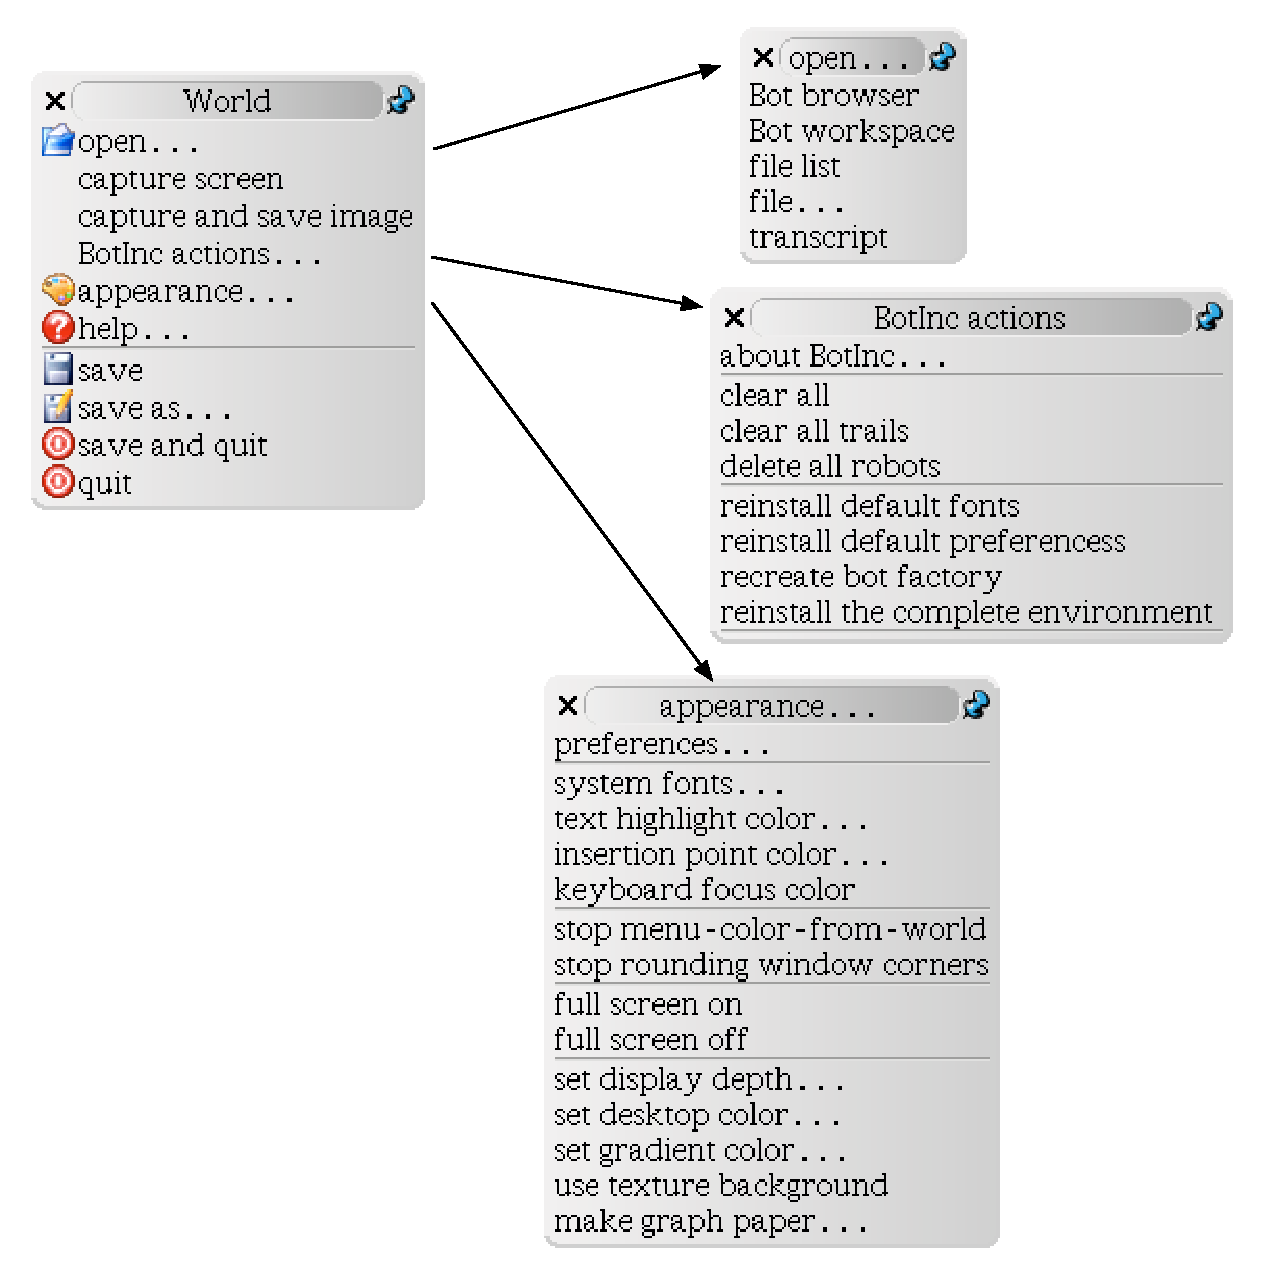
\includegraphics[width=8cm]{allMenu}
\caption{Menu options of the environment.\label{fig:allMenu}}
\end{center}
\end{figure}

If you want to know what each menu item does, simply let the mouse pointer on it for one second, a balloon should pop up describing the item. The main menu gives access to five main groups of functionalities: access to tools, screen capture, access to some robot behavior, appearance,  and saving the environment. The submenus are grouped as follows: 

\begin{itemize}
\item[open...] The menu \button{open...} groups several tools such as the robot code browser, the \tw, a file browser and other tools that I will present when needed
\item [BotInc actions] The menu \button{BotInc actions} groups several actions such as indicating the version of the environment, clear all the robots and their traces, but also some actions to reinstall the environment if needed: reinstall default preferences set back the default preferences that you may have modified using the following menu. 
\item [appearance] The menu \button{appearance...} groups actions related to change the appearance of the environment such as the fonts used, the full screen mode, the color of the background.
\end{itemize}


\paragraph{Getting a \tw.}
It may happen that you close the default \tw. This is not a problem as you can get a new one easily from the dark blue flap as shown by Figure~\ref{fig:caroflaps} or from the main menu as shown before. To install a new \tw in the working flap, open the working flap (bottom flap) and drop the bot workspace from the blue flap into the bottom flap. 

\begin{figure}
\begin{center}
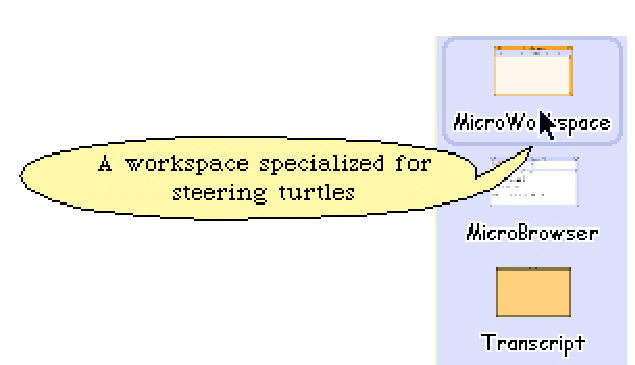
\includegraphics[width=7cm]{smallcaroflap}\hfill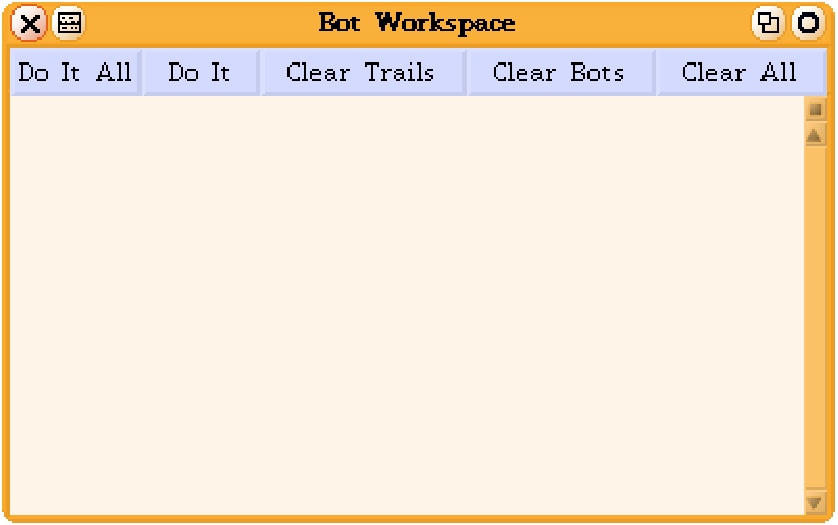
\includegraphics[width=7cm]{FullTurtleWorkspace}
\caption{Getting a new \tw from the flaps. \label{fig:caroflaps}}
\end{center}
\end{figure}

The dark blue flap contains other tools that we are going to use in the future. Basically, the second tool is a code browser that you will use when you will define new robot methods. 


\section{Interacting with \sq}
\sq interaction is based on the assumption that you have a three button mouse. Each button is associated with a logical set of operations. The left button is for pointing and selecting, the middle button is for window manipulation (bringing a window in front, moving it), and the right button for bring context sensitive menu and handles which are small colored and round buttons floating around graphical elements (as shown in Figure~\ref{fig:rohals}). The handles are useful as they allow you to interact directly with the robot. I will present them in detail in the next chapter.  

\begin{figure}[h]
\begin{center}
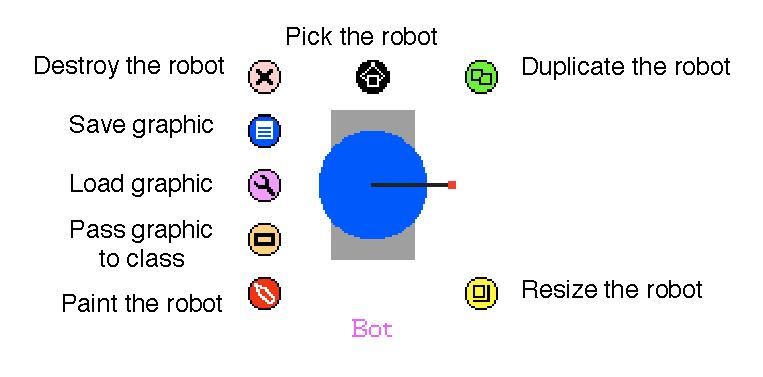
\includegraphics[width=8cm]{picaAllHaloAnnotated}
\caption{Right-clicking on a robot brings its handles.\label{fig:rohals}}
\end{center}
\end{figure}


Depending on your machine, you will need to click with different mouse button and key combinations as explained by the following table: 

\begin{center}
\begin{tabular}{|| p{2.5cm} | p{3cm} | p{3cm} | p{3cm} ||} \hline \hline
Button:           &   Left       &    Center       &  Right \\ \hline \hline
Kind of Actions:  &  Pointing, selecting     & Context    sensitive menu  &   Bringing halos \\ \hline
Windows 2-Button  Equivalent&   Left-Click    & Alt-Left    &   Right Click \\ \hline
Mac 1 Button  Equivalent&  Click      &    Option-click &  Cmd-Click \\ \hline 
\hline
\end{tabular}
\end{center}


\section{Using \tw to Save a Script}
The \tw has 5 buttons and also a menu that allows you to save scripts.
The button \textbf{Do It All} executes the entire script that the workspace contains.
The button \textbf{Do It} executes the part of the script that is currently selected in  the workspace. The button \textbf{Clear Trails} clears only the robot trails without removing the robots themselves. The button \textbf{Clear Robots} removes only the robots without cleaning their trails. The button \textbf{Clear All} removes all the robots and their trails.

Once you have written a script you may wish to save to a file  for future uses. The \tw provides a way of saving and loading files via its menu. 

\begin{figure}[h]
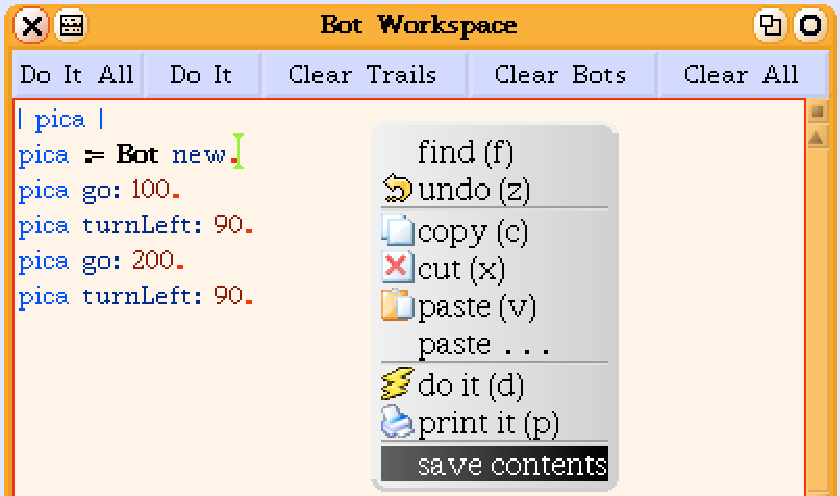
\includegraphics[width=7cm]{saveContents}
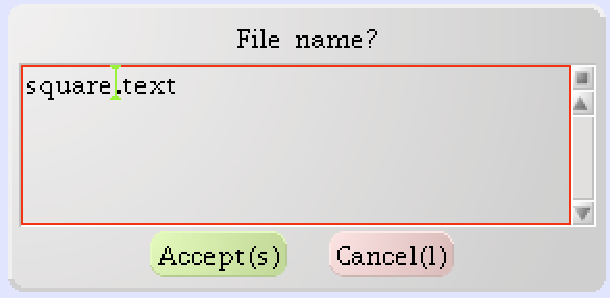
\includegraphics[width=4cm]{enteringFileName}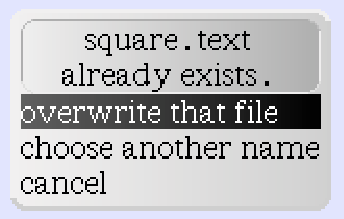
\includegraphics[width=4cm]{overwrite}
\caption{\tw menu options.  Middle: Specifying the name of the file in which the script is saved. Right: When the file already exist you can overwrite it or rename it.\label{fig:turtleMenu}\label{fig:enteringFileName}}
\end{figure}

Click on the contents of the workspace to bring up its associated menu as shown in Figure~\ref{fig:turtleMenu}. The menu item \menu{save contents} will save the complete contents of the workspace into a file. Selecting this menu item brings up a dialog box as shown in Figure ~\ref{fig:enteringFileName}. Note that the system checks whether a file with the same name already exists or not. If such a file already exists, the system asks you if the file should be overwritten or to provide another name as shown in Figure ~\ref{fig:enteringFileName}.


\section{Loading a Script}
To load a script, you have to use a \index{file list} \fl, a tool that allows you to select and load different files into \sq. You can obtain a file list by selecting the menu item \button{open...} and \button{file list} from the main menu.  A \fl is composed of several panes. The top left pane allows you to navigate the volumes and folders, each time you select an item in this pane the top right pane is updated. It shows all the files contained in the folder you selected in the left pane. When you select a file in the right pane, the bottom pane automatically shows its contents. Figure~\ref{fig:filelistOpen} shows we are in  the folder \ct{Bot testing} in  which  the file \ct{square.text} is selected. 


%\begin{figure}
%\begin{center}
%\includegraphics[width=6cm]{fileListInFlap}\caption{The FileList thumbnail available in the Advanced Flap. \label{fig:fileListInFlap}}\end{center}
%\end{figure}


\begin{figure}[h]\begin{center}
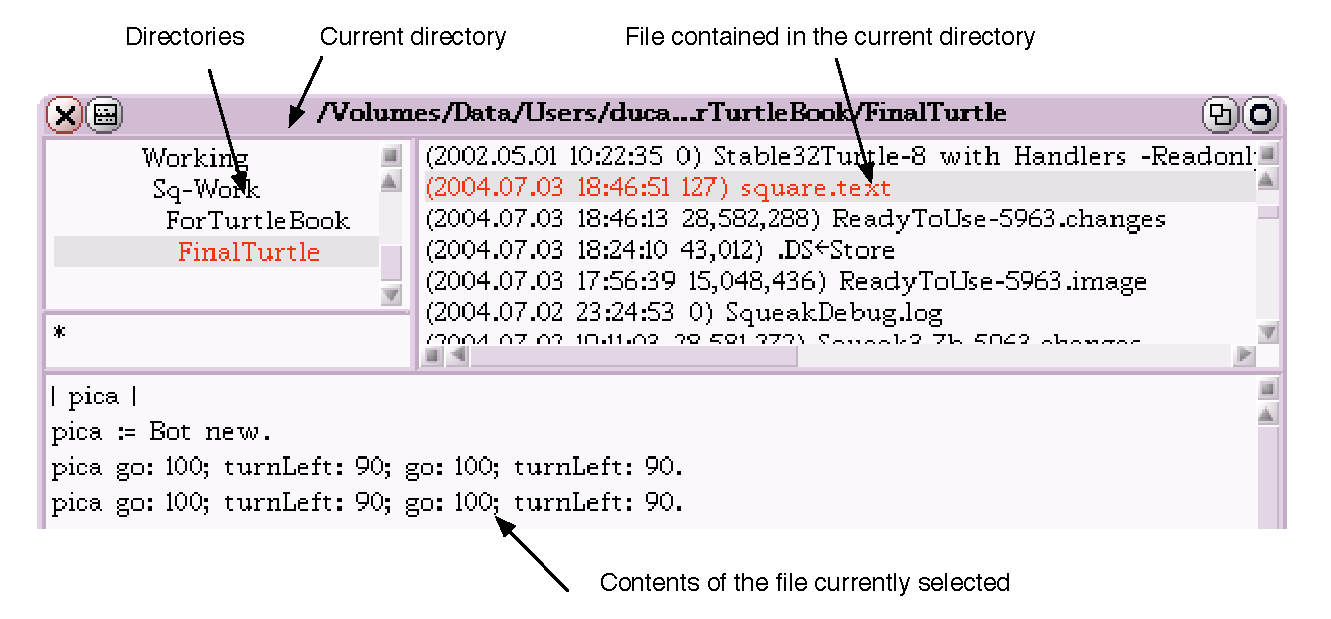
\includegraphics[width=12cm]{filelistOpenAnnotated}
\caption{The \fl opened on the script named \ct{square.text}.\label{fig:filelistOpen}}\end{center}
\end{figure}

To load a script you simply have to copy  the contents of the bottom pane using the menu item (\menu{copy}) and paste  (\menu{paste}) it into the \tw as you would do with any texteditor.   





%\begin{figure}
%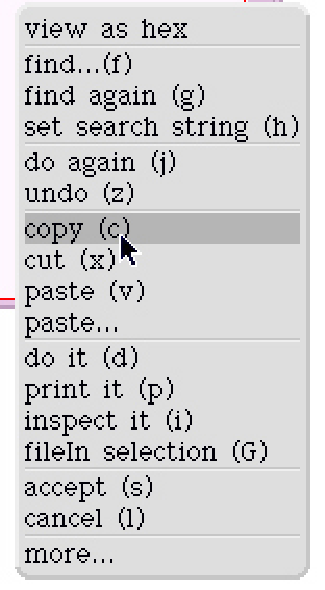
\includegraphics{copyFromFileList}
%\end{figure}




\section{Capturing a Drawing}
To keep a trace of your drawings you can use the screen capture of your computer. However, on certain computers you may have problem to get a screen capture. To avoid this problem, the environment proposes a simple screen capture mechanism that works on any computer. Bring the main menu by clicking on the background of the environment. The menu offers two items named: \menu{capture screen} and \menu{capture and save image} as shown by Figure~\ref{screenCapture}. 

The easier way is to use the \menu{capture and save image} menu item. When you select this item \sq shows that it is ready to capture by changing the cursor to be like a corner as shown by Figure~\ref{screenCapture}. Place the cursor and click at the corner of the rectangular region you want to capture, hold down the menu and move the mouse to delimit the region you want. The region is shown in the bottom left corner and \sq prompts you to get the name of the file without extension that it will save.

\begin{figure}[h]
\begin{center}
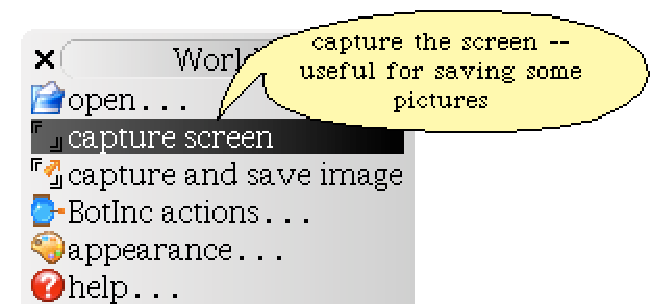
\includegraphics[width=7cm]{screenCapture} 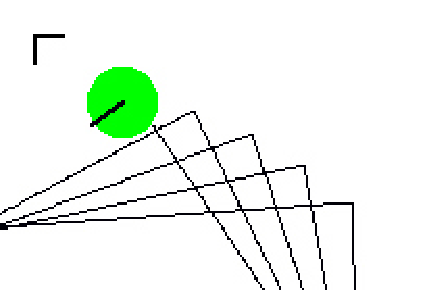
\includegraphics[width=7cm]{positioningScreen}
\caption{Left: Two possibilities to capture and save the capture. Right: The cursor is changed. \sq is ready for the capture. Now click to position one corner of the rectangular region you want to capture.}\label{screenCapture}
\end{center}
\end{figure}


Now you may want to sort and choose the screen captures that you want to keep. For that you can capture a region of the screen using the menu item \menu{capture screen}. In such a case \sq will not prompt you to save the file, but instead it creates a picture on the \sq desktop.  Then you can save it by bringing the handles by right-clicking on it. You should get different handles around the image as shown by Figure~\ref{sketchWithHalo}. Once the halos are there around your image, click on the red handle which brings a menu of actions that you can apply on the image. Select the \menu{export...} item and the format in which the image will be save. \sq will prompt you for the name of the file. Note that you can import in \sq these files by dropping them from the desktop into the \sq desktop. 



\begin{figure}
\begin{center}
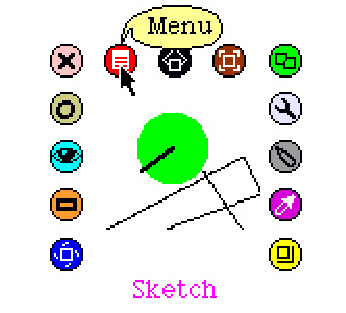
\includegraphics[width=4cm]{sketchWithHalo}
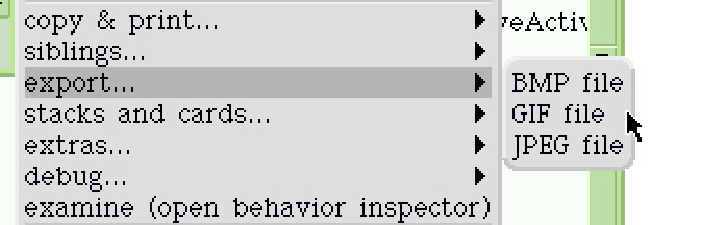
\includegraphics[width=9cm]{sketchExportMenu}
\caption{Bring the halos and chose the red halo menu item \menu{export...} to save the image on disk.} \label{sketchWithHalo}
\end{center}
\end{figure}




\section{Message Result}
In \st, objects only communicate by receiving from and sending messages to other objects. Once an object receives a message it executes it and it may return a \index{result} \emph{result}. A result is an object that you get back from a message.
In a similar fashion that for some letters that we receive, we need to perform actions and for others we need to sign an acknowledgment that we effectively received the letter. 

For example sending the message \ct{go: 100} to a robot asks the robot to move 100 pixels in its current direction. But there is no result returned. In certain cases the result of a message execution is important. For example, sending the message \ct{+ 3} to the object \ct{2} returns \ct{5}. Sending the message \ct{color} to a robot returns its current color. The result of a message is important to be able to compose multiple messages. For example, when the expression \ct{(2+ 3) * 10} is executed, the expression \ct{(2 + 3)} returns \ct{5}. This number is then used in another message \ct{* 10} which finally returns \ct{50}.

\cadre{A result is an object that you get from a message. 

\begin{nalltt}
2 + 5 \\
    returns 7\\
pica color\\
    returns its color, a color object
\end{nalltt}}

The \sq environment allows you to \textit{execute messages} without taking care of the message's result, or execute messages \textit{and print the returned message value}. If the difference is not really clear the following example illustrates it. Imagine that you have a small robot that carries items. When you tell him to move, the robot will just move but you will not get anything back. Now if you ask the robot to give you an item, it will execute this order by moving one of its physical elements \textit{and} gives you the item.  This example illustrates the difference between executing a message and executing a message that returns a value. 

\paragraph{Vocabulary Point.} In \sq jargon printing an result means giving an ascii (character-based) format version of the result just after the expression and not on a physical printer. In Figure~\ref{fig:printitMenu} \ct{140} is composed of three characters that represent the number one hundred forty and one hundred fifty is the result returned by the sum of the number fifty and ninety.

\begin{figure}[h]
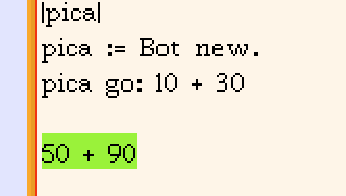
\includegraphics[width=5cm]{selectingExp}  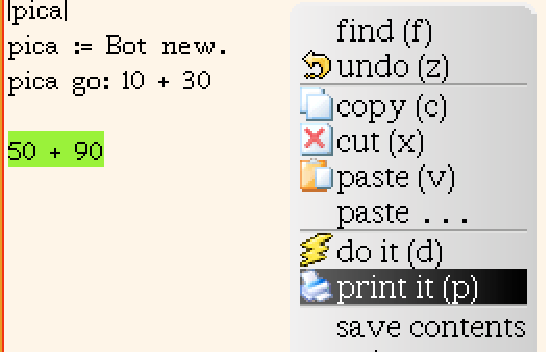
\includegraphics[width=5cm]{selectMenu}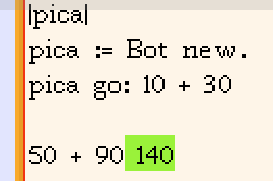
\includegraphics[width=5cm]{resultExpression}
\caption{Left: Selecting the expression \ct{50 + 90}. Middle: Bringing the menu. Right: Executing it and getting the result printed.\label{fig:printitMenu}}
\end{figure}


Now there are three ways of executing a script.
\begin{enumerate}
\item Using the buttons of the \tw editor.  In \charef{cha:firstscript} I show you a simple way to execute your first code by pressing the \button{Do It All} button of the \tw. But to execute a script you can also \emph{select} the text you want to execute with the mouse (the selection goes green) and you press the \button{Do It} of the \tw.

\item Using the menu. Select the part of your script you want to execute as shown by \index{executing} Figure~\ref{fig:doitMenu}, get the menu by pressing  the middle button of your mouse (or press the option key while clicking with the left button), then  chose the \menu{do it (d)} or the \menu{print it (p)} menu item as shown by the Figure~\ref{fig:printitMenu}. 

\item Using keyboard shortcuts. Select a piece of text, then press command-d on mac and alt-d on PC).
\end{enumerate}



\paragraph{Hints.} To automatically select all the text, you can just click at the start of the text (before the first character) or at the end of the text, or on the line after the last expression.  If you want to select a word, you can just double-click anywhere on the word.  If you want to select a line just double-click at the beginning (before the first character) or end (after the last character) of the line.

 
\begin{figure}[h]
\begin{center}
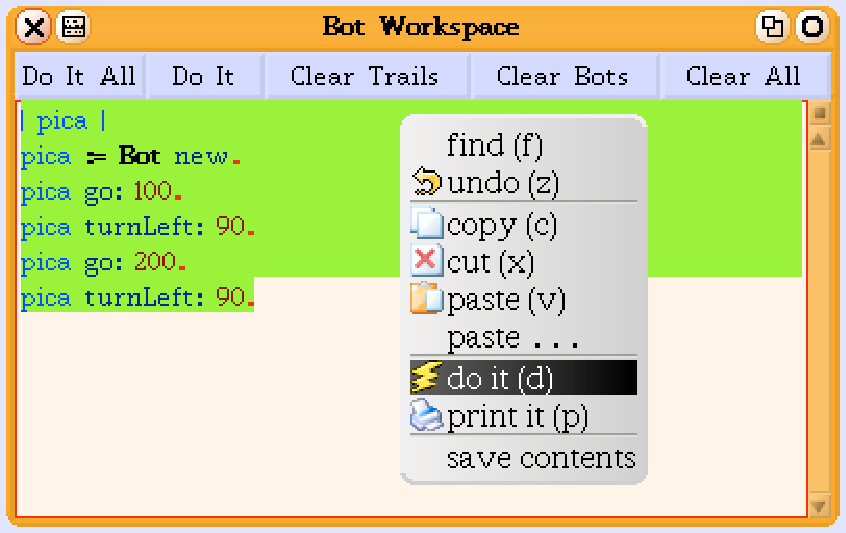
\includegraphics[width=8cm]{doitViaMenu}
\caption{Selecting a piece of a script and executing it explicitly using the menu.\label{fig:doitMenu}}
\end{center}
\end{figure}


\paragraph{Two Examples.}
When you execute the message \ct{\caro color} which asks the robot its color using the \menu{do it (d)} menu item, the message is effectively sent and executed. However, you have the impression that nothing happens. This is because you do not ask the system to take care about the result of the message execution. When you are interested by the result of a message you should use the menu item \menu{print it (p)} as shown by Figure~\ref{fig:colorPrintIt}. This has the effect to execute the piece of code selected \emph{and} print the result returned by the last message composing the code.
Here the message \ct{\Turtle new} is executed, then the message \ct{color} is sent to the newly created robot. The message \ct{color} is executed and the color of the receiving robot is returned and printed as shown by Figure~\ref{fig:resultColorPrintIt}.
 \ct{(TranslucentColor r: 0.0 g: 0.0 b: 1.0 alpha: 0.847)} tells us that the color of the robot is a transparent color composed from the three color component red, green and blue.






\begin{figure}
\centerline{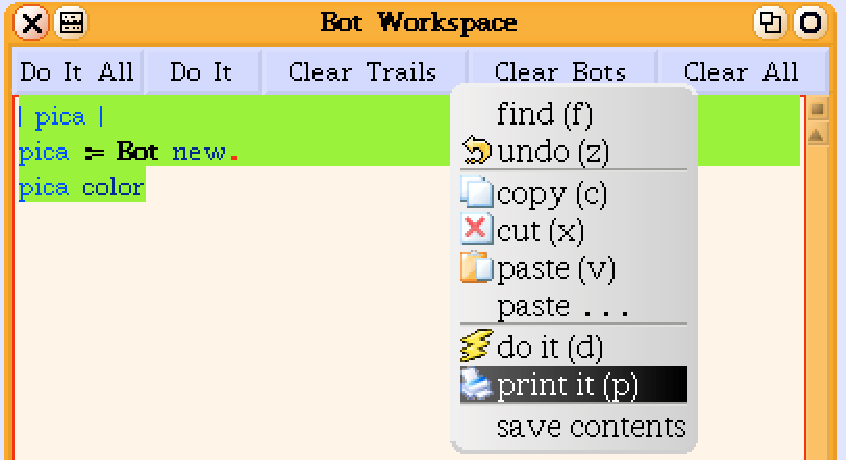
\includegraphics[width=8cm]{colorPrintIt}} 
\caption{Bring the menu and select the menu item \menu{Print it (d)} to execute the selected piece of code \textit{and} print the returned result.\label{fig:colorPrintIt}}
\end{figure}

\begin{figure}
\centerline{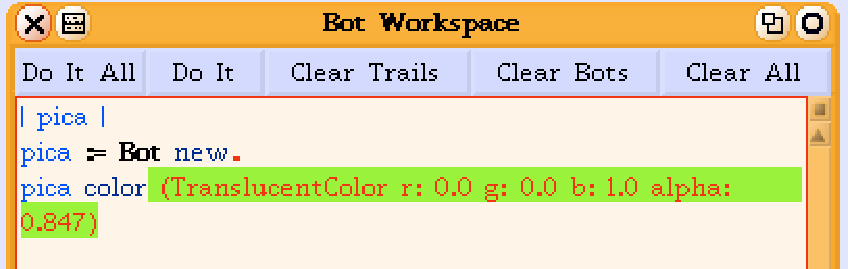
\includegraphics[width=8cm]{resultColorPrintIt}} 
\caption{Bring the menu and select the menu item \menu{Print it (d)} to execute the selected piece of code \textit{and} print the returned result.\label{fig:resultColorPrintIt}}
\end{figure}

Let's look at a final example to make sure that you understand when to use  \menu{print it}. When you execute the message \ct{100 + 20} using the menu item \menu{do it (d)}, the message \ct{+ 20} is effectively sent to the object \ct{100} that adds \ct{20}. However you do not see anything. This is normal because in  such a case the execution of the \ct{+} message returns a new number representing the sum but you did not ask \sq to print it. To see it you have to print the result of the message execution using the menu item \button{Print It}. From now  we will use \pr to indicate that we use the \menu{print it} to get the message executed and its result printed as shown in the scripts \ref{scr:doitprint}. Note that we will only use this convention when the result is important. 


\begin{scriptwithtitle}{Printing the result of an expression execution}\label{scr:doitprint}
(100 + 20) * 10
\pr 1200
\end{scriptwithtitle}


\begin{largecadre}{There are two ways of executing an expression: using the \menu{Do It} menu item to execute an expression. Using the   \menu{Print it} menu item to  execute it and print the returned result.}
\end{largecadre}




\summa
\begin{itemize}
\item \emph{To execute an expression}. Select a piece of text representing one or several expression and press the \button{Do It} button or select the menu item
\menu{do it} from the execution menu.

\item A result is an object that you get from a message. For example, \ct{pica color} returns the color of the robot.

\item There are two ways of executing an expression: using the \menu{Do It} menu item to execute an expression. Use the   \menu{Print it} menu item to  execute it and print the returned result.

\end{itemize}


\ifx\wholebook\relax\else\end{document}\fi



